\documentclass[12pt]{article}
\pagestyle{plain}
\usepackage{amsmath}
\usepackage{bm}
\usepackage{graphicx}
\usepackage{wrapfig}
\graphicspath{ {./} }
\usepackage{float}
\usepackage{setspace}

\doublespacing

\begin{document}

\title{PhD Candidacy Proposal: \\
A Strategy for a Single-Photon Source Using a Kerr-Cavity Weakly
Coupled to a Quantum Emitter}
\author{c praise anyanwu 
    \thanks{anyanc@uw.edu} \\
    Chemistry Department, University of Washington
}
\date{14 December 2022}
\maketitle

\newpage
\section{Introduction}
Encoding information in the quantum state of a single photon (using degrees
of freedom of polarization, momentum, or energy) is highly desirable in 
secure quantum communication since photons travel at the speed of light and 
interact weakly with the environment over long distances.
\cite{gisin2002quantum, bennett2004quantum} For example, in the quantum key 
distribution protocol, Alice encodes information in the qubit of a photon 
polarization state. \cite{bennett1984proceedings, bennett1992quantum}
Importantly, if Alice must securely transmit this qubit through a quantum 
channel to Bob, and without loss of information to an eavesdropper, then 
Alice's single-photon source must be deterministic. A deterministic 
single-photon source emits a single photon \textit{on demand}, with $100 \: 
\%$ probability. In practice, one evaluates the single-photon nature of a 
source by the ratio of the probability of single-photon to multi-photon 
emission. \cite{lounis2005single, eisaman2011invited}

%Single-photon sources can be categorized between two main classes.
%\cite{lounis2005single, eisaman2011invited} The former lies towards a
Deterministic single-photon sources involve effective two level systems 
(quantum dots, single atoms, single ions) \cite{ShieldsAndrewJ2007Sqls, 
strauf2007high, hennrich2004photon, wilk2007single, maurer2004single} 
that emit a single photon when excited by a resonant incident field. 
Less deterministic single-photon sources involve nonlinear processes as 
parametric down conversion in waveguides (or four-wave mixing in optical 
fiber systems) \cite{u2004efficient, sharping2001observation, 
goldschmidt2008spectrally} that emit a correlated pair of photons, where 
one photon heralds the other. The known difficulties with these systems 
involve trapping of a single ion or atom strongly coupled to cavities at 
cryogenic temperatures for deterministic single-photon sources, while 
care must be taken for less deterministic sources in order to avoid 
generating multiple pairs of photons. Herein, we propose a theoretical 
basis for a novel single-photon source that circumvents both 
ion-trapping at ultra-cold temperatures and the need for strong 
coupling. The measure of the system's single-photon nature is based on 
the calculated second order correlation function of transmitted light.

Consider the following system: a high-Q cavity coupled to a broad-band 
emitter. For example, ref. \cite{pan2019elucidating} has an emitter placed 
on the chip of a toroidal silica microcavity with a $10^{7}$ Q-factor 
(Fig. 1a). We propose the following modification: a quantum emitter placed 
on a Kerr-cavity coated with polystyrene, which has a significant 
$10^{- 12} \:\mathrm{cm}^2/\mathrm{W}$ third-order nonlinear 
susceptibility. \cite{qin2010design, liu200910} (Polystyrene's third-order 
nonlinearity originates from the delocalization of the $\pi$-conjugated 
electrons along the polymer chains. \cite{krausz1989optical, 
wong1991studies}) This achieves a Kerr effect such that the resonance of 
the nonlinear cavity now depends on the photon-number in the cavity 
(Fig. 1b).

\begin{figure}
  \centering
  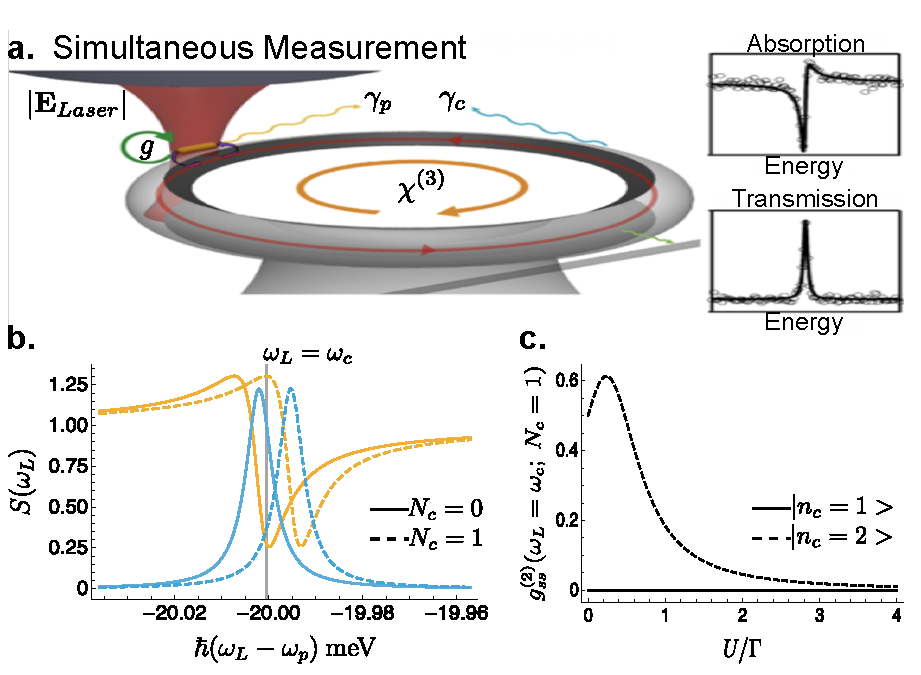
\includegraphics[width=1\linewidth]{fig.pdf}
  \caption{(a) Example of the proposed experimental set-up
  \cite{pan2019elucidating}, which in general, consists of a broad-band
  quantum emitter (here represented as gold nanorod) placed unto\textemdash
  and weakly coupled to\textemdash a Kerr-cavity (here represented as
  toroidal micro-ring resonator). The emitter is pumped with a
  laser, and its absorption spectrum shows a Fano profile due
  to its interaction with the high-Q cavity. At the vicinity of the
  anti-resonance, there is a peak in transmission of light through the cavity
  out-coupled to the measuring fiber optic cable. (b) The spectral distribution
  of the reduced average photon-number in the broad-band mode at steady-state
  $\langle b^{\dagger}b \rangle_{ss}/\langle b^{\dagger}b \rangle_{ss; g=0}$,
  yellow curves, and the average photon number in the discrete cavity mode 
  of a single-photon state $\langle n_c=1\vert \: a^{\dagger}a \:
  \vert n_c=1 \rangle_{ss}$, blue curves. 
  The solid curves are the spectra when the cavity has zero-photon
  occupation $N_c=0$, while the dashed curves, the cavity has a single-photon
  occupation $N_c=1$. (c) The second order correlation calculated at steady
  state when the cavity is populated with a single-photon occupation.
  The single-photon blockade is eviedent for a Kerr-nonlinearity whose value is
  withtin the order of the Fano line-width, i.e., $\chi^{(3)} \propto U=\Gamma$.
  }
  \label{fig}
\end{figure}

A characteristic of the coupled Kerr-cavity-emitter system is the cavity 
photon-number dependent Fano resonance, with a resonant peak and 
anti-resonant dip corresponding to an enhanced and diminished absorption by the
emitter (see Fig. 1b). Just at the vicinity of the  anti-resonance, there is 
transmission of a photon into the cavity. Upon single-photon population, the
Kerr-cavity resonance is detuned from a pump laser exciting the system at the
anti-resonance. And if the kerr-cavity resonant frequency shift is on the order 
$\Gamma$ (the FWHM equal to the line-width between the anti-resonant dip and 
the resonant peak of the Fano Profile), then the system experiences a 
single-photon blockade, as shown in the calculated $g^{(2)}_{ss}$ (Fig. 1c) 
of light transmitted through the cavity at steady state. Thus the single-photon 
blockade effect depends on the Fano resonance shift $\Delta\omega$ induced by the 
Kerr-cavity's non-linearity, where the degree of nonlinearity that induces the 
shift $\Delta\omega$ is proportional to $\Gamma$, such that,
\begin{equation}
\begin{split}
\omega_1 - \omega_0 &= (\omega_0 + \Gamma ) - \omega_0
\\
\Delta\omega &= \Gamma
\end{split}
\end{equation}
with $\omega_{0,1} = c n_{0,1} k$, and $n_1$ is the refractive index due
to the kerr effect \cite{spillane2002ultralow}:
\begin{equation}
\begin{split}
n_1 &= n_0 + n_2 I
\\
&= n_0 + \frac{3 \chi^{(3)}}{8 n_0 c\epsilon_0} I.
\end{split}
\end{equation}
Note that $n_2$ is the value often reported for the third-order susceptibility,
such that the Kerr effect is induced by the local intensity $I$ from the pump 
laser populating the kerr-cavity. From the above equations we find the relation:
\begin{equation}
\begin{split}
\frac{\Delta \omega}{ck} &= n_2 I \\
\end{split}
\end{equation}
For a cavity mode $\lambda \approx 1566 \:\mathrm{nm}$,
\cite{pan2019elucidating, heylman2013photothermal} with a third-order 
susceptibility $n_2 \approx 1.15 \times 10^{-12} \:\mathrm{cm}^2/\mathrm{W}$, 
\cite{qin2010design} the desired blockade effect can be achieved for a 
single-photon state whose resonance is shifted by $\Delta\omega \approx 
\Gamma$, if the local intensity $I \ge 7.41 \: \mathrm{MW}/\mathrm{cm^2}$, 
which is the regime of a faint laser beam whose coherent state could have an 
average photon-number in the range $\mu = 0.1-2$. \cite{al2008characterization}
This is advantageous because the desired blockade effect could be achieved with 
a faint laser beam or with a kerr-cavity of much smaller $n_2$.


\section{Model}
We develop the system's dynamics in Heisenberg picture. Heisenberg picture is 
suitable to calculate the quantum statistical correlation of the field of light 
transmitted through the Kerr cavity. This field correlation can be related to 
the experimentally observed spectral distribution, using the spectral response 
function. \cite{scully1999quantum} Moreover, in the Heisenberg picture the 
dynamics of the quantum transverse field is analogous to the classical 
transverse field \cite{tannoudji1992atom}, which allows for direct comparison 
to the classical system. \cite{pan2019elucidating} Then damping of the 
single-mode in the cavity field (and of the broad-band field) is described 
using Heisenberg-Langevin formalism. In so doing, this model provides a simple 
yet rigorous quantum approach (complementing the Louivillian formalism in the
Linblad form, recently developed in Ref. \cite{finkelstein2015fano, 
finkelstein2016nonlinear}) to account for damping of the discrete state 
(cavity mode) of Fano resonance, and the spectral distribution derived from 
this model is expressed in terms of Fano-parameters. \cite{fano1961effects}

The Hamiltonian of the discrete Kerr-cavity coupled to a broad-band emitter is
the following: $\mathcal{H} = \mathcal{H}_{a} + \mathcal{H}_{b} + 
\mathcal{H}_{f} + \mathcal{H}_{I}$. The derived Hamiltonian $\mathcal{H}_{a}$ 
is the energy of a single-mode dielectric Kerr-cavity in free space 
\cite{jackson1999classical, hillery1984quantization}, such that,
\begin{equation}
\begin{split}
\mathcal{H}_{a} &= \frac{1}{2} 
    \int_{V} \mathrm{d}^{3}\mathbf{x} \: \mathbf{P} \cdot \mathbf{E}
\\
&= \frac{1}{2} 
    \int_{V} \: \mathrm{d}^{3}\mathbf{x}
    \Big( \mathbf{P}^{(1)} + \mathbf{P}^{(3)} \Big)
    \cdot \mathbf{E}
\\
&= \frac{1}{2} 
    \int_{V} \: \mathrm{d}^{3}\mathbf{x} \: 
    \Big( \bm\chi^{(1)} \mathbf{E}  + 
    \frac{3}{4}\bm\chi^{(3)}:\mathbf{E}\mathbf{E}^{*} \mathbf{E} \Big)
    \cdot \mathbf{E}
\end{split}
\end{equation}
where $3/4\mathbf{\chi}^{(3)}$ is the higher order nonlinear susceptibility of
a Kerr-cavity \cite{butcher1990elements}, and the quantized field $\mathbf{E}$
is normalized with respect to the cavity's mode volume $V$. In the rotating
wave approximation (and for a linear polarization), $\mathcal{H}_{a}$
simplifies as follows
\begin{equation}
\begin{split}
\mathcal{H}_{a} &= \pi\hbar\omega_k \Big(
    \chi^{(1)}_{ef} +
    \frac{3}{4} \chi^{(3)}_{ef} \mathcal{E}^2
    a^{\dagger}a + \frac{3}{4}\bm\chi^{(3)} \mathcal{E}^2 : \mathbf{1} \Big)
    \Big( a^{\dagger}a + \frac{1}{2} \Big)
\\
&= \hbar \Big( \omega_c + U\:a^{\dagger}a \Big)
    \Big( a^{\dagger}a + \frac{1}{2} \Big)
\\  
&\approx \hbar \Big( \omega_c + U \langle a^{\dagger}a \rangle \Big)
    \Big( a^{\dagger}a + \frac{1}{2} \Big).
\end{split}
\end{equation}
where $\mathcal{E} = \sqrt{2\pi \hbar \omega_k / V }$ is the amplitude of the
quantized field.

The first-order approximation in Eq. (5) linearizes the nonlinear term.
This is based on the motivation that the resonant frequency of a kerr-cavity
changes as a function of intensity $|\mathbf{E}|^2$. In this case, the resonant
frequency depends on the average photon-number in the Kerr-cavity:
\begin{equation}
\omega_c^{NL}( N_c = \langle a^{\dagger}a \rangle )  = \omega_c + UN_c.
\end{equation}
Thus the Hamilonian for the single-mode Kerr-cavity $\mathcal{H}_a$, the 
bosonic broad-band field $\mathcal{H}_b$, and the free field $\mathcal{H}_f$
is as follows:
\begin{align}
\mathcal{H}_a &= \hbar\omega_c^{NL}
    \Big( a^{\dagger}a + \frac{1}{2} \Big),
\\
\mathcal{H}_b &= \hbar\omega_p
    \Big( b^{\dagger}b + \frac{1}{2} \Big),
\\
\mathcal{H}_f &= \hbar \sum_j \omega_j
    \Big( f^{\dagger}_j f_j + \frac{1}{2} \Big).
\end{align}
The discrete cavity mode $\omega_c^{NL}$ and the broad-band mode $\omega_p$
both disipate energy to the free fields $\omega_k$. Thus the interaction
Hamiltonian $\mathcal{H}_{I}$ is as follows:
\begin{equation}
\mathcal{H}_I = \hbar g \: (
    a^{\dagger}b + b^{\dagger}a )
    + \hbar \sum_j ( V_j^a f^{\dagger}_j a 
        + V_j^b f^{\dagger}_j b + \mathrm{h.c.} ).
\end{equation}
We work in Purcell regime where $|V_a| \ll g \ll |V_b|$. Note that the
original Fano problem is the limit where $|V_a| \rightarrow 0$.

Deriving the Heisenberg-Langevin equation of motion for the slowly varying
operator $A = a \: e^{i\omega_c^{NL} t}$, and then 
transforming back to the non-slowly varying operator $ a = 
A \: e^{-i\omega_c^{NL} t}$ yields
\begin{align}
\dot{ a } &= -i ( \omega_c^{NL} - i\gamma_c/2 ) a 
    - ig b,
\\
\dot{b} &= -i ( \omega_p - i\gamma_p/2 ) b
    - ig a,
\end{align}
$\gamma_{c,p}$ accounts for both radiative and non-radiative damping as
described in Ref \cite{thakkar2015quantum}. (Note that the above equation
has assumed an evacuated initial reservoir state.)

In the experiment, the broad-band mode is driven by the external
field of a monochromatic laser operating at $\omega$. The spectral 
distribution is derived from the spectral response function, such that,
\begin{equation}
S(\omega) = \frac{1}{\pi} \int_0^{\infty} \mathrm{d}\tau \: 
    e^{i \omega \tau} 
    \langle b^{\dagger}(t_0=0) \: b(t_0 + \tau) \rangle.
\end{equation}
We find that the spectral response function can be interpreted as the steady 
state solution of the average photon-number in the broad-band mode rotating 
in the frame of the drive frequency, i.e.
\begin{align}
S(\omega) &= \langle \tilde{b}^{\dagger}_{ss}\tilde{b}_{ss} \rangle
\\
\tilde{b}^{\dagger}_{ss} &= 
    b^{\dagger}_{ss} \: e^{i \omega_L t}; \quad
    \tilde{a}^{\dagger}_{ss} =
    a^{\dagger}_{ss} \: e^{i \omega_L t};
\\
\dot{b}_{ss} &= 0 =
    -i ( \omega_p - i\gamma_p/2 ) b_{ss} - ig a_{ss}
    + iE_{Laser}( e^{i \omega_L t} - e^{-i \omega_L t} ).
\end{align}
and $E_{Laser}$ is the amplitude of the monochromatic laser operating at
a drive frequency $\omega = \omega_L$. The reduced spectral response yields
\begin{equation}
\begin{split}
\frac{ S(\omega = \omega_L) }{ S(\omega = \omega_L)_{g=0} } &= 
    \frac{\langle \tilde{b}^{\dagger}_{ss}\tilde{b}_{ss} \rangle}
        {\langle \tilde{b}^{\dagger}_{ss}\tilde{b}_{ss} \rangle}_{g=0}
\\
&= \Bigg( 1 +
    \frac{\gamma_c}{\gamma_p}
    \frac{g^2}{(\omega_L - \omega_c^{NL})^2 + (\gamma_c/2)^2}
    \Bigg) \:
    \left\vert \frac{q + \epsilon}{\epsilon + i} \right\vert^2.
\end{split}
\end{equation}
The first term is the Fano profile, where 
$\epsilon=(\omega_L - \omega_{eff})/(\gamma_{eff}/2)$ and 
$q = (\omega_c^{NL} - i\gamma_c/2 - \omega_{eff})/(\gamma_{eff}/2)$;
%$\omega_{eff}$, $\gamma_{eff}$, and $q$ are the Fano parameters. The second
$\epsilon$ and $q$ are the Fano parameters. The second
term is the Lorentz distribution due to the line-width broadening of the
discrete state. The spectral distribution reduces to the Fano profile in the
limit $\gamma_c \propto |V_a| \rightarrow 0$.

Since we are interested in single-photon blockade due to the Kerr-nonlinearity, 
$U \propto \chi_{eff}^{(3)}$, we calculate the second order
correlation function $g^{(2)}_{ss}$ of light transmitted through the Kerr-cavity
coupled to the driven broad-band emitter, at the steady state, as a function
of U, i.e.,
\begin{equation}
\begin{split}
g^{(2)}_{ss}(U) &\equiv 
    \frac{ \langle n_a, n_b \vert \:
    \tilde{a}^{\dagger}_0 \: \tilde{a}^{\dagger}_{ss}(U)
    \tilde{a}_{ss}(U) \: \tilde{a}_0 \:
    \vert n_a, n_b \rangle }
    {(\langle \tilde{a}^{\dagger}_0\tilde{a}_0 \rangle)^2}
\\
&= \frac{g^2}{n_a}
    \frac{\langle n_a-1 \vert \: E_{Laser}^2 \: \vert n_a-1 \rangle}
    {\left\vert \big( \omega_L - \omega_c^{NL}(U) + i\gamma_c/2 \big)
    \big( \omega_L - \omega_p + i\gamma_p/2 \big)
    -g^2 \right\vert^2}.
\end{split}
\end{equation}
%\begin{equation}
%\begin{split}
%g^{(2)}_{ss}(U) &\equiv 
%    \frac{ \langle n_a, n_b \vert \:
%    \tilde{a}^{\dagger}_0 \: \tilde{a}^{\dagger}_{ss}(U)
%    \tilde{a}_{ss}(U) \: \tilde{a}_0 \:
%    \vert n_a, n_b \rangle }
%    {(\langle \tilde{a}^{\dagger}_0\tilde{a}_0 \rangle)^2}
%\\
%&= \frac{n_a \langle n_a - 1, n_b \vert \:
%    \tilde{a}^{\dagger}_{ss}\tilde{a}_{ss} \:
%    \vert n_a - 1, n_b \rangle}
%    {n_a^2}
%\\
%&= \frac{1}{n_a} 
%    \frac{g^2}
%    {\left\vert \omega_L - \omega_c^{NL}(U) + i\gamma_c/2 \right\vert^2}
%    \langle n_a - 1, n_b \vert \:
%    \tilde{b}^{\dagger}_{ss}\tilde{b}_{ss} \:
%    \vert n_a - 1, n_b \rangle
%\\
%&= \frac{g^2}{n_a}
%    \frac{\langle n_a-1 \vert \: E_{Laser}^2 \: \vert n_a-1 \rangle}
%    {\left\vert \big( \omega_L - \omega_c^{NL}(U) + i\gamma_c/2 \big)
%    \big( \omega_L - \omega_p + i\gamma_p/2 \big)
%    -g^2 \right\vert^2}.
%\end{split}
%\end{equation}
For single-photon blockade, the photon-number in the cavity is set to one,
such that, $\omega_c^{NL}( U, N_c = 1 )  = \omega_c + U$. Importantly, the
amplitude of the laser field to populate the bare ($N_c=0$) cavity mode 
with a single photon at steady state is such that
\begin{equation}
\begin{split}
\langle n_a=1 \vert \:
    \tilde{a}^{\dagger}_{ss} \tilde{a}_{ss} \:
    \vert n_a=1 \rangle 
    &= n_a = 1
\\
&= \frac{ g^2 \: 
    \langle n_a \vert \: E_{Laser}^2 \: \vert n_a \rangle}
    {\left\vert \big( \omega_L - \omega_c^{NL}(N_c=0) + i\gamma_c/2 \big)
    \big( \omega_L - \omega_p + i\gamma_p/2 \big)
    -g^2 \right\vert^2}.
\end{split}
\end{equation}
thus, it follows that
\begin{equation}
\langle n_a \vert \: E_{Laser}^2 \: \vert n_a \rangle = n_a
    \left\vert 
    ( i\gamma_c/2 )( \omega_c - \omega_p + i\gamma_p/2 ) -g^2 
    \right\vert^2
    / g^2.
\end{equation}


\section{Previous work}
%%Graphical TOC
%\begin{wrapfigure}{r}{0.5\textwidth}
%  \begin{center}
%    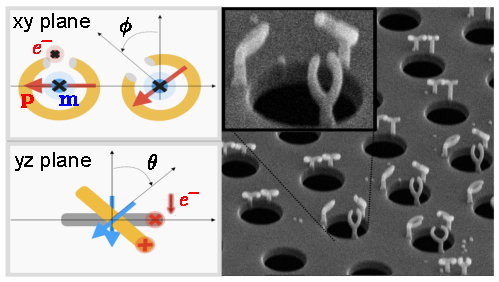
\includegraphics[scale=1.0]{./cavity_study/toc_graphicv4.pdf}
%  \end{center}
%  \caption{Graphical TOC}
%\end{wrapfigure}
Previous work focuses on individual cavities. \cite{pakeltis2019focused}
We design and characterize split ring resonator (SRR) cavities arranged 
in a dimer or trimer array. Due to the split of the ring, and the 
circular current path of the ring, these SRR cavities exhibit both 
electric and magnetic dipoles. We map out the electric $g_E$, magnetic 
$g_H$, and overall interaction strength 
$G = \vert g_E \vert \cos\phi - \vert g_B \vert \cos\theta$, 
and its effect on the normal mode energy splitting 
$G_{eff} = \left\vert G/\Omega_0 \right\vert$, between coupled 
SRR dimers, as a function of the spatial degrees of freedom\textemdash
exploring both the two-dimensional in-plane rotaion $\phi$ 
(Fig. 2, Table 1), and the three-dimensional out-of-plane tilt $\theta$ 
(Fig. 2, Table 2).
%Graphical TOC
\begin{figure}[H]
  \begin{center}
    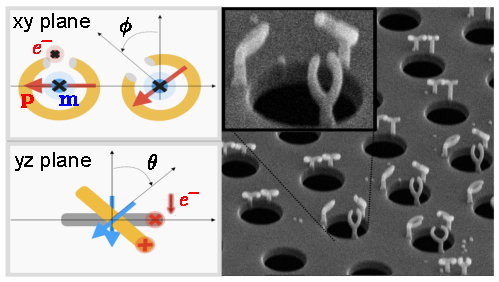
\includegraphics[scale=1.0]{./cavity_study/toc_graphicv4.pdf}
  \end{center}
  \caption{Graphical TOC: This work is currently under review at 
  ACS Optical Applied Materials.}
\end{figure}
This study is the first to characterize the third-dimensional (3D) degree of 
freedom, where the analysis of the EEL probability shows that for a particular
orientation, increasing the 3D tilt angle $\theta$ diminishes the magnetic 
coupling, but enhances the overall light-matter interaction strength. 

%%2D
%\begin{figure}
%    \centering
%    \includegraphics[width=1.0\textwidth]{./cavity_study/eels_srrsbs2d.png}
%    \caption{
%    (a) Experimental (solid), simulation (circle), and model (dashed) 
%    EEL spectra taken at the SRR outer tip for planar rotational study. 
%    (b-f) HAADF images of each SRR dimer with a colored circle indicating 
%    where the spectra in panel a were acquired. Corresponding spectrum 
%    images show the lower-energy (g-k) and higher-energy (l-p) normal 
%    modes of the system. Scale bar = 300 nm.} 
%\label{fig:2drotate}
%\end{figure}
%%3D
%\begin{figure}
%  \centering
%  \includegraphics[width=0.5\linewidth]{./cavity_study/eels_srrsbs3d.png}
%  \caption{EEL spectra of individual coupled 3D SRR dimers. 
%  For each dimer, the SRRs are placed side-by-side. 
%  (a) Experimental (solid) and model (dashed) EEL spectra, with the 
%  electron probe placed at one of the SRR's outer tips. The electron 
%  probe is represented as a color-coded circle in the HAADF image, 
%  corresponding to each color-coded spectrum. For the blue curves, the 
%  3D out-of-plane tilt ($\theta$) angles are $30^{\circ}$-$30^{\circ}$, 
%  respectively, for the electron probe driven-undriven SRRs in the dimer, 
%  while for the red curves the $\theta$ angles are 
%  $30^{\circ}$-$45^{\circ}$, respectively. (b) The planar orientation 
%  for the SRR dimer is as such in Fig. \ref{2drotate}d, and then the EEL 
%  spectra are acquired for same the 3D tilt orientations conducted in (a).
%  }
%  \label{3drotate}
%\end{figure}

%Table 2D
\begin{table}[H]
	\centering
	\caption{2D Parameter estimates}
	\label{table:parameters}
	\begin{tabular}{ c c c c }
		\hline\hline
 		\multicolumn{0}{}{} $A \: 
        [\mathrm{s^2\cdot cm^{-1}}]$ & $\hbar\omega_0$ [meV]
 		& $\hbar|g_E|$ $[\mathrm{meV^2}]$ & $\hbar|g_H|$ $[\mathrm{meV^2}]$ \\
 		\hline
 		$1.885 \times 10^{-31}$ & $359$
 		& $6.5 \times 10^{-2}$ & $9.0 \times 10^{-3}$ \\
 		\hline \\ [0.01ex]
 		\hline
 		$\phi$ [deg] & $\hbar\Omega_0$ [meV]
 		& $\hbar\gamma_0$ [meV] & $\hbar|G_{\textrm{eff}}|$ $[\mathrm{meV}]$ \\
 		\hline
 		$0$ & $362$ & $47$ & $65$ \\
 		$45$ & $360$ & $47$ & $54$ \\
 		$90$ & $359$ & $47$ & $25$ \\
 		$135$ & $365$ & $55$ & $64$ \\
 		$180$ & $370$ & $58$ & $82$ \\
 		\hline\hline
	\end{tabular}
\end{table}
% 3D
\begin{table}[H]
	\centering
	\caption{3D Parameter estimates}
	\label{table:parameters3d}
	\begin{tabular}{ c c c c c c}
		\hline\hline
 		\multicolumn{0}{}{} $\phi$\ [deg] & $\theta$ [deg]
 		& $\hbar\Omega_0$ [meV] & $\hbar\gamma_0$ [meV]
 		& $\hbar|G_{\textrm{eff}}|$ [meV] & $\hbar\omega_0$ [meV] \\
 		\hline
 		$0$ & $0$ & $389$ & $52$ & $33$ & $410$ \\
 		$0$ & $15$ & $387$ & $51$ & $85$ & $\sim$ \\
 		$90$ & $0$ & $390$ & $78$ & $20$ & $\sim$ \\
 		$90$ & $15$ & $404$ & $48$ & $15$ & $\sim$ \\
 		\hline\hline
	\end{tabular}
\end{table}

Based upon the model provided in this work, we additionally examine the 
hybridization of individual 2D SRR trimers measured using EELS. 
Taken together, this study elucidates the geometric effects of 3D tilt on 
the SRR magnetic dipole moment and its role in the hybridization of 
coupled 3D SRRs, thus serving as a stepping stone for nano-engineering 
NIR metamaterials composed of coupled 3D SRR units. This work is currently 
under review at ACS Optical Applied Materials.
%%Trimer Figure.
%\begin{figure}
%    \centering
%    \includegraphics[width=0.8\textwidth, height=0.8\textheight, 
%    keepaspectratio]{./cavity_study/planartrimer_v4.pdf}
%    \caption{
%    EEL point spectra, spectrum images, and induced electric and magnetic 
%    field profiles of a planar SRR trimer with $D_{3h}$ symmetry. 
%    (a) HAADF image of the trimer. Scale bar = 300 nm. (b) Experimental 
%    EEL spectra acquired at the beam positions indicated in panel a. 
%    (c-d) Experimental spectrum images at the resonant energies of 
%    300 meV and 400 meV with FM and AFM ordering, respectively, shown in 
%    the simulated field profiles of (e) the electric dipole in-phase 
%    lower-energy normal mode, (f) the electric dipole out-of-phase 
%    higher-energy normal mode, (g) the magnetic dipole in-phase lower-energy 
%    normal mode, (h) the magnetic dipole out-of-phase higher-energy normal mode.} 
%    \label{fig:trimer}
%\end{figure}


\newpage
\bibliography{ref_database}
\bibliographystyle{unsrt}

\end{document}
